\documentclass{beamer}
\usepackage{pgfpages}
\usepackage{newtxtext,newtxmath} %time new roman
%\setbeameroption{show notes}
%\setbeameroption{show notes on second screen=right}
\usetheme{Warsaw}
\usepackage[french]{babel}

\usepackage{tikz}
\pgfdeclareimage[height=0.5cm]{le-logo}{}
%\setbeamertemplate{footline}[frame number]
%Set number slide
\usepackage[backend=biber, natbib, maxbibnames=20, citestyle=authoryear]{biblatex}
\addbibresource{handwritten.bib} 
\usepackage{multirow}% row fusion
\usepackage{array} % column fusion
\usepackage{xfrac} % small fractions
\usepackage{adjustbox}
\usepackage{listings}
\usepackage{color}
\definecolor{gray}{rgb}{0.4,0.4,0.4}
\definecolor{darkblue}{rgb}{0.0,0.0,0.6}
\definecolor{cyan}{rgb}{0.0,0.6,0.6}
 \titlegraphic{\vspace{-1cm}
      
\includegraphics[width=2.5cm]{images/paris8_1}\hspace*{4.75cm}~%
      \hfill
      
\includegraphics[width=2.5cm]{images/logo}
}
\setbeamertemplate{frametitle}{\nointerlineskip  
    \begin{beamercolorbox}[wd=\paperwidth,ht=2.75ex,dp=1.375ex]{frametitle}
        \hspace*{2ex}\insertframetitle \hfill {\small\insertframenumber/\inserttotalframenumber} \hspace*{1ex}%
    \end{beamercolorbox}}

\usecolortheme{wolverine}
\setbeameroption{hide notes} % Only slides


%%%%%%%%%%%%%%%%%%%%%%%%%%%
\title[Reconnaissance de caractères manuscrites] 
{Off-Line Handwritten Character Recognition System Using Support Vector Machine}
%\subtitle {ne compléter que si l'article possède un sous-titre}
\author[Komlan Dantodji] 
{Komlan Jean-Marie DANTODJI}

\institute[]
{
  Etudiant en M1 Big Data
  \and
  Université Paris 8}
\date{26 novembre 2020}


\begin{document}
\begin{frame}
  \titlepage
\end{frame}

\begin{frame}{Plan}
  \tableofcontents
\end{frame}
\section{Introduction à la méthode du SVM : Support Vector Machine}
\subsection{Linéarité séparable}
\begin{frame}{Linéarité séparable}
	\begin{figure}[H]
    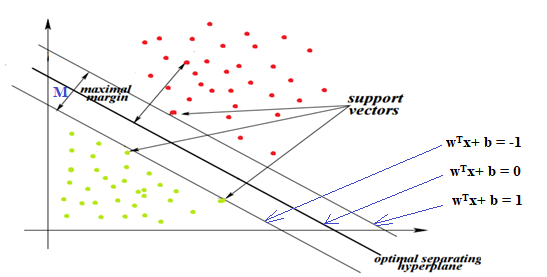
\includegraphics[width=\linewidth]{images/svm_separate.png}
    \caption{Détermination de l’hyperplan}
    \label{fig:L1}
\end{figure}
\end{frame}

\subsection{Déterminsation d'hyperplan}
\begin{frame}{Déterminsation d'hyperplan}
 $x_0$ et $x_1$ deux vecteurs supports aux deux extrémités,\\
Soit l' hyperplant $$(P): w^Tx+b=0$$

$$M = d(x_{0},P)+d(x_{1},P) = \frac{\mid{w^{T}x_{0}+b}\mid}{\sqrt{w^{T}w} } + \frac{\mid{w^{T}x_{1}+b}\mid}{\sqrt{w^{T}w} } $$

$$ = \frac{\mid{1}\mid}{\sqrt{w^{T}w} } + \frac{\mid{-1}\mid}{\sqrt{w^{T}w}} = \frac{2}{\sqrt{w^{T}w} }$$  
\par Maximiser M revient à minimiser $$\frac{\sqrt{w^{T}w}}{2} = \frac{\|w\|}{2}$$
\end{frame}
\begin{frame}{Déterminsation d'hyperplan}
\par Maximiser M revient à minimiser $$M=\frac{\sqrt{w^{T}w}}{2} = \frac{\|w\|}{2}$$
\end{frame}

\subsection{Linéarité inséparable}
\begin{frame}{Linéarité inséparable}
\begin{figure}[H]
    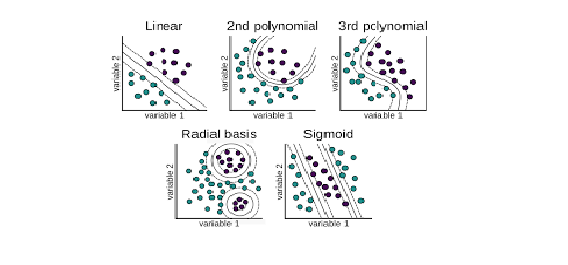
\includegraphics[width=\linewidth]{images/svm_non_linear.png}
    \caption{Inséparabilité linéaire : https://www.r-bloggers.com/2019/10/support-vector-machines-with-the-mlr-package/}
    \label{fig:L1}
\end{figure}
\end{frame}
\subsection{Linéarité inséparable}
\begin{frame}{Fonctions Kernel}
Kernel linéaire: $$  K(X_{i},X_{j})=x_i^T x_j$$\\
Kernel Polynomial:  $$K(X_i,X_j ) = (\gamma x_i^T x_j+r)^d$$\\
Kernel Radial: $$K(X_i,X_j ) = \mathrm{e}^{\gamma(x_i-x_j )^2}$$\\
Kernel Sigmoid: $$K(X_i,X_j )= \tanh{(\gamma x_i^T x_j+r)}$$
\end{frame}


\section{Etapes de prétraitement:}
\subsection{Etapes de traitement d'image de texte manuscrit}
\begin{frame}{Les étapes de prétraitement} 
\begin{itemize}
		\item Binarization 
		\item Slant Correction
		\item Smoothing and Noise Removal 
		\item Size Normalization
\end{itemize}
\end{frame}
\subsection{Shema des étapes}
\begin{frame}{Shéma des étapes} 
\begin{figure}[H]
    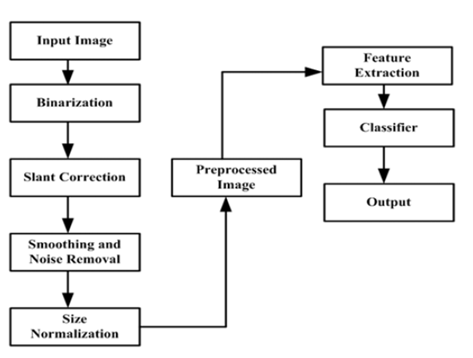
\includegraphics[width=9cm,height=5.5cm]{images/pretraitement.png}
    \caption{Etapes de prétraitement de l’image : http://www.sciencepublishinggroup.com/j/ajnna}
    \label{fig:L1}
\end{figure}
\end{frame}
\subsection{Extraction des caractéristiques}
\begin{frame}{Extraction des caractéristiques} 
\begin{figure}[H]
    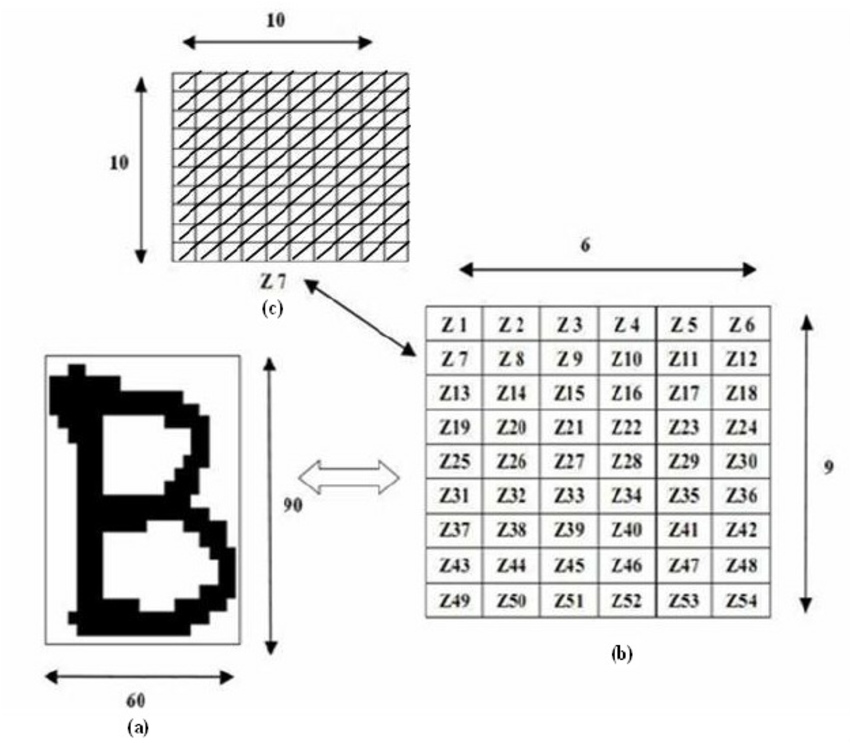
\includegraphics[width=12cm,height=5.2cm]{images/diagonal_methode.png}
    \caption{Méthode d'extraction diagonale: https://www.researchgate.net/figure/Procedure-for-extracting-feature}
    \label{fig:L1}
\end{figure}
\end{frame}


\section{Model de SVM }
\begin{frame}{Les différents étapes de SVM } 
\begin{figure}[H]
    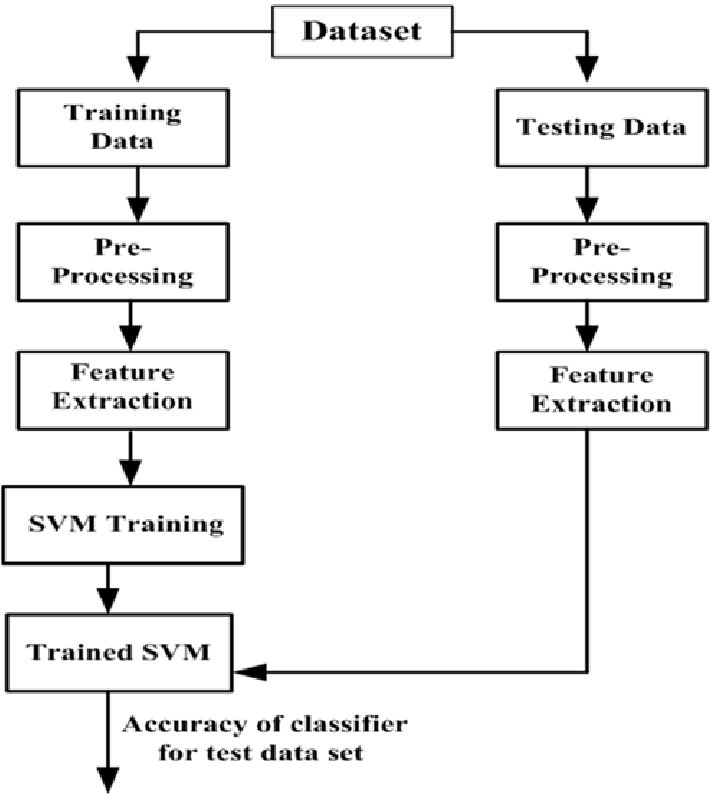
\includegraphics[width=9cm,height=5.5cm]{images/svm_methode.png}
    \caption{Etapes de SVM: https://www.researchgate.net/figure/Different-stages-of-SVM-classification}
    \label{fig:L1}
\end{figure}
\end{frame}


\section{Synthèse et Conclusion}
\begin{frame}{Synthèse et Conclusion}
\begin{figure}[H]
    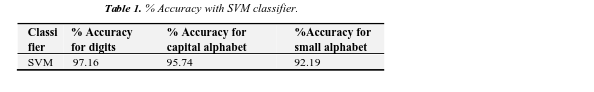
\includegraphics[width=15cm,height=4cm]{images/accuracy.png}
    \caption{https://www.researchgate.net/publication/323112207Off-Line Handwritten Character Recognition System Using Support Vector Machine}
    \label{fig:L1}
\end{figure}
\end{frame}

\end{document}